\documentclass[12pt]{article}
\usepackage[a4paper, total={6in, 10in}]{geometry}
%\usepackage[top=0in, bottom=1in, left=1.25in, right=1.25in]{geometry}


\usepackage{enumitem}   
\usepackage{url}
\usepackage{graphicx}
\graphicspath{{figs/}} 


\title{Quantifying Complexity of Facial Expressions 
Variability with Nonlinear Dynamics
in Human-Humanoid Interaction} 
\author{Miguel Xochicale\\ 
}
\date{21th December 2018}

\begin{document}
\maketitle
%\thispagestyle{empty} %No number


\begin{abstract}
This research proposal aims to investigate the use of a method from nonlinear dynamics 
(RQAEnt) to quantify the complexity of face expressions variability and 
its relationship with mental states (e.g. anxiety, disinterest, relief)
in the context of human-humanoid interaction. 
The proposal contains two research questions,
an introduction to RQAEnt, and a pilot experiment with preliminary results.
\end{abstract}


\section{Introduction}
Movement variability is an inherent feature within and between persons. 
Research on measurement and understanding of movement variability has been 
well established in the last three decades in areas such as biomechanics, 
sport science, psychology, cognitive science, neuroscience and recently
in human-robot interaction \cite{2018arXiv181009249X}.
Hence, considering methodologies for movement variability 
to quantify complexity of facial expressions variability 
with its preliminary experiments \cite{MPXochicale_CERE2018},
I am therefore interested in quantifying the complexity 
of facial expression for a person and in researching 
the subtle variations of facial expressions that can be related to different 
mental states (e.g. anxiety, disinterest, relief, etc.)  \cite{back2014}
both in the context of human-humanoid interaction.
Such statements have led me to ask two research questions for this
proposal: 
\begin{enumerate}[label=(\roman*)]
 \item does the quantification of the complexity of facial expressions 
	variability can tell us something about the state of mind of a person?, 
\item how the quantification of facial expressions can be related with 
the complexity of facial expressions?.
\end{enumerate}

\section{Methods}
Considering the work of my Ph.D. thesis where I investigated nonlinear dynamics
to quantify movement variability in 
human-humanoid interaction \cite{XochicalePhDThesis2018},
I am therefore proposing to apply Recurrence Quantification Analysis (RQA) to
give little insights into the raised questions.
RQA computes measurements based on the recurrence points density of diagonal 
or vertical line structures in Recurrence Plots \cite{marwan2007}. 
Such measurements can provide understanding of the dynamics of a system 
i.e. the determinism (predictability) or Shannon entropy (complexity).
Hence, with the use Shannon Entropy with RQA (also known as RQAEntr),
one can quantify the complexity of face expressions variations. 

\section{Preliminary results}
Fig \ref{fig:method} shows the proposed methodology 
where one participant (myself) were asked to perform three levels of 
face expressions:
(i) neutral variation, (ii) slow variation and (iii) faster variations.
Figs \ref{fig:method}(B) shows the time series from the $x$ 2D landmarks
for normalised and smoothed time series.
It can be noted from the time series an increase of amplitude and 
variations as the face expressions varies. I can hypotheses that 
such changes can be related to subtle variation of face expressions
and therefore related with the state of mind of a person. 
Hence, Fig \ref{fig:method}(C) shows a 3D surface of the RQAEnt 
in $z-axis$ with embedding values in $x-axis$ and 
recurrence thresholds in $y-axis$ 
that quantify the complexity of face expressions 
(see \cite{2018arXiv181009249X} for RQAEnt).


%%---------------------------------(FIGURE)-------------------------------------
\begin{figure}
\centering
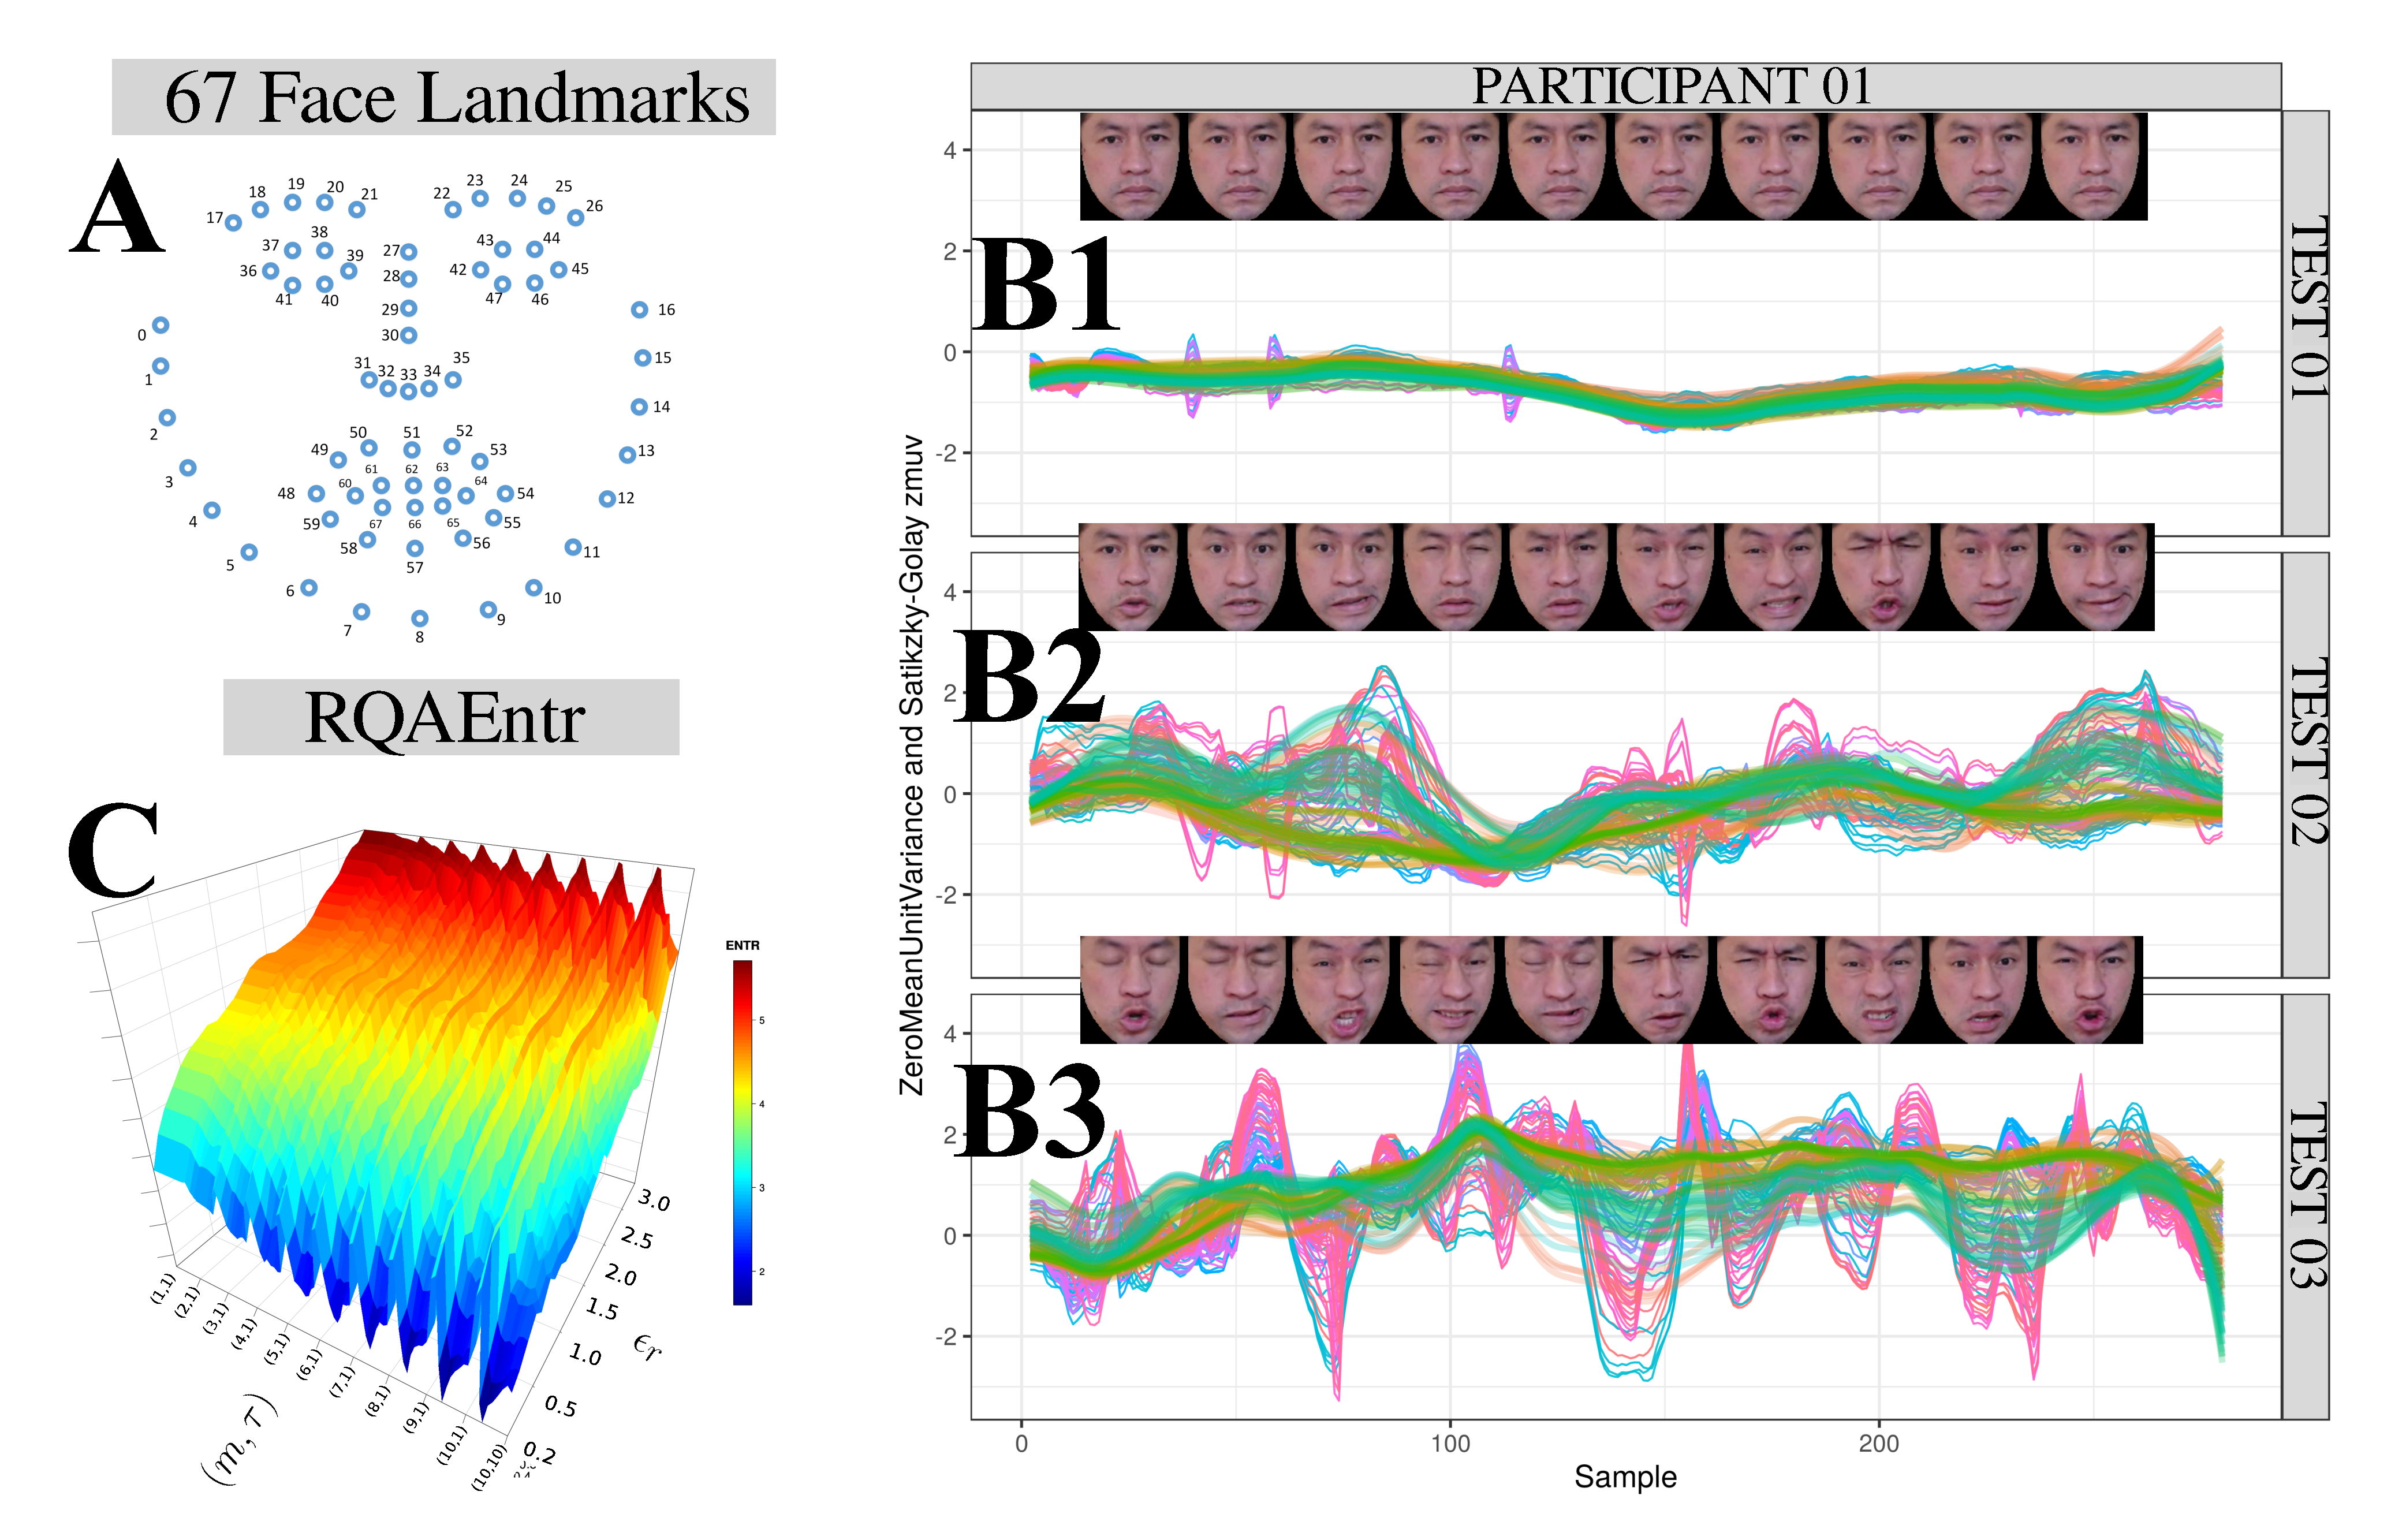
\includegraphics[width=1.0\textwidth]{main/method}
    \caption{
	{\bf Dynamics of face landmarks variations.}
	{\bf(A)} 67 2D face landmarks (FL) with OpenFace \cite{baltrusaitis2018}.
	Time series and faces with vertical lines for: 
	{\bf(B1)} neutral face expressions,
	{\bf(B2)} slowly variation of face expressions, and
	{\bf(B3)} faster variation of face expressions.   
	{\bf(C)} 3D surface of RQAEntr for $x$ 2D landmark position over time.
	R code to reproduce the figure and the results 
	is available from \cite{xochicale2018repo}.
        }
\label{fig:method}
\end{figure}
%%---------------------------------(FIGURE)------


\bibliographystyle{alpha}
\bibliography{references/references}


\end{document}
